\RequirePackage{luatex85}
\documentclass[tikz]{standalone}

\usetikzlibrary{mindmap, arrows.meta}
\begin{document}

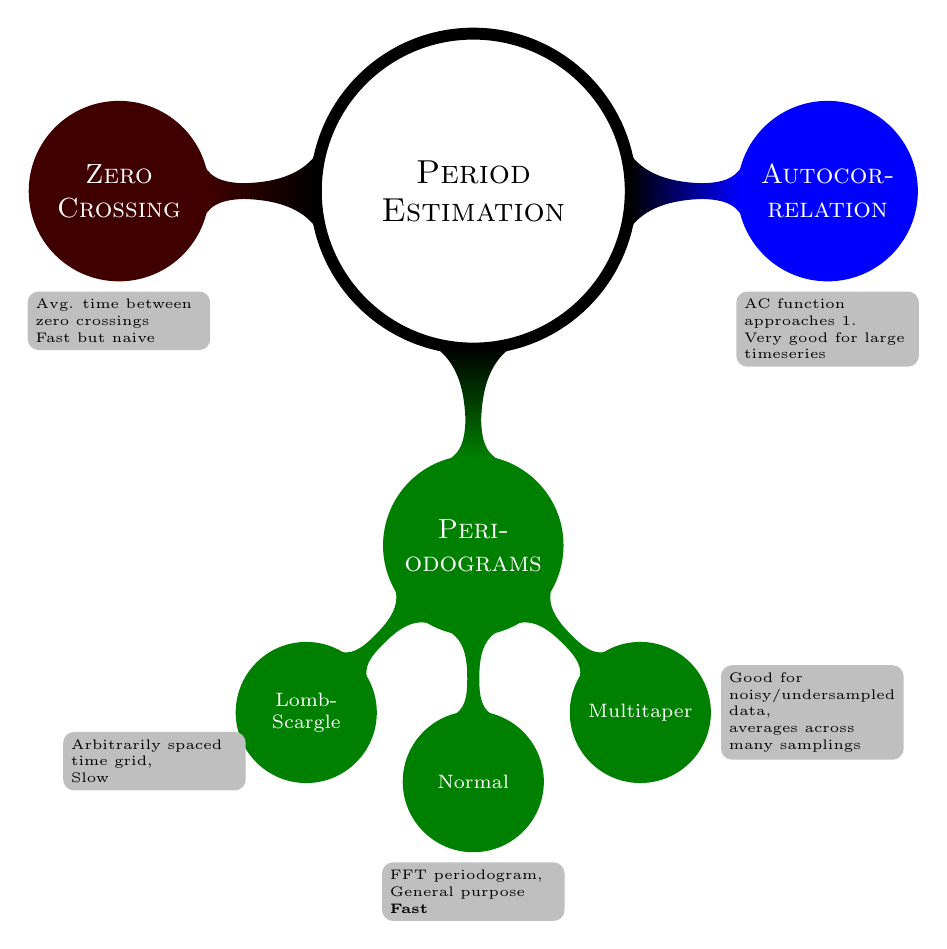
\begin{tikzpicture}[
      mindmap
  ]

  \begin{scope}[
      every node/.style={concept, execute at begin node=\hskip0pt},
      root concept/.append style={concept color=black, fill=white, line width=1ex, text=black, font=\large\scshape},
      text=white,
      autocor/.style={concept color=blue,faded/.style={concept color=blue!50}},
      zc/.style={concept color=red!25!black,faded/.style={concept color=red!25!black!50}},
      periodogram/.style={concept color=green!50!black,faded/.style={concept color=green!50!black!50}},
      grow cyclic,
      level 1/.append style={level distance=4.5cm,sibling angle=90,font=\scshape, clockwise from=0}, level 2/.append style={level distance=3cm,sibling angle=45,font=\scriptsize, clockwise from=-45}
  ]

      \node [root concept, align=center] {Period\\Estimation} % root
        child [autocor] { node (Autocor) {Autocorrelation}}
        child [periodogram] { node (Periodograms) {Periodograms}
          child { node (Multitaper) {Multitaper} }
          child { node (Normal) {Normal} }
          child { node (Lomb-Scargle) {Lomb-Scargle} }
        }
        child [zc] {node (zc) {Zero Crossing}};
  \end{scope}

  \begin{scope}[
    every node/.style = {annotation},
    every annotation/.style = {fill=gray!50!white, text width = 14ex}
    ]

    \node [right] at (Multitaper.east) {Good for noisy/undersampled data,\\averages across many samplings};
    \node [below] at (Normal.south) {FFT periodogram,\\General purpose\\\textbf{Fast}};
    \node [left] at (Lomb-Scargle.south west) {Arbitrarily spaced time grid,\\Slow};

    \node [below] at (zc.south) {Avg. time between zero crossings\\Fast but naive};
    \node [below] at (Autocor.south) {AC function approaches 1.\\Very good for large timeseries};

  \end{scope}

\end{tikzpicture}

\end{document}
